%!TEX root = ../template.tex
%%%%%%%%%%%%%%%%%%%%%%%%%%%%%%%%%%%%%%%%%%%%%%%%%%%%%%%%%%%%%%%%%%%%
%% dmem_scour_application.tex
%% NOVA thesis document file
%%%%%%%%%%%%%%%%%%%%%%%%%%%%%%%%%%%%%%%%%%%%%%%%%%%%%%%%%%%%%%%%%%%%

\typeout{NT FILE dmem_scour_application.tex}

\chapter{Application of the DMEM Strategy to Scour-Induced Capacity Degradation}
\label{cha:dmem-scour-application}

The previous chapters introduced and validated the \gls{DMEM} strategy for the structural assessment of masonry arch bridges under vertical loading. This chapter presents the next step of the PhD work: the application of that validated numerical strategy to a flood-related damage mechanism, namely local scour at bridge foundations.

The purpose of the chapter is not to develop a hydraulic scour model. The hydraulic and temporal aspects of scour are discussed in \Cref{cha:state-of-art}. Instead, the focus here is structural: given an idealised loss of foundation support, the objective is to understand how the bridge redistributes forces, how the governing mechanism changes, and how the residual load-carrying capacity degrades. This information is required for later fragility and decision-support developments because it links a flood-induced physical process to structural performance indicators.

\section{Motivation and Scope}
\label{sec:dmem-scour-motivation}

Flood-induced local scour is one of the most critical threats to masonry arch bridges because many of these structures rely on shallow foundations and are sensitive to differential settlements \cite{Kirby2015,Tubaldi2018}. In practical bridge management, scour vulnerability is often assessed through geometric or conservative criteria, for example by assuming critical conditions when scour reaches the foundation base. Such criteria are useful for screening, but they do not explicitly quantify the residual structural capacity of a bridge subjected to partial support loss, nor do they explain how the location and extent of scour affect collapse mechanism formation.

The validated \gls{DMEM} model provides a suitable basis for addressing this gap. It is able to reproduce the mechanisms of masonry arch bridges, including flexural rocking, sliding, pier displacement, and three-dimensional interaction between bridge components, while remaining computationally efficient enough for repeated scenario analyses. In this chapter, the method is applied to a representative three-span masonry arch bridge previously used in the validation campaign \cite{Melbourne1997,Bonatte2026DMEM}. The analysis is deliberately simplified to isolate the structural consequences of support degradation.

The specific objectives are:

\begin{enumerate}
    \item to extend the validated \gls{DMEM} model by introducing a simplified soil--foundation interaction;
    \item to represent progressive scour through controlled removal of soil--foundation support;
    \item to quantify the residual load-carrying capacity for different scour locations and severities;
    \item to identify the governing collapse mechanisms and their dependence on pier kinematics;
    \item to clarify the role of this type of analysis within the broader PhD framework for flood risk and resilience assessment.
\end{enumerate}

\section{Reference Bridge}
\label{sec:dmem-scour-reference-bridge}

The reference structure is the three-span masonry arch bridge tested by Melbourne et al. \cite{Melbourne1997}. The bridge consists of three 3 m spans and two intermediate piers. The same bridge was analysed in the \gls{DMEM} validation campaign described in \Cref{cha:dmem-validation}, where the numerical model was compared with experimental and numerical benchmark results. This makes it an appropriate case study for extending the validated model to support-degradation scenarios.

\begin{figure}[htbp]
\centering
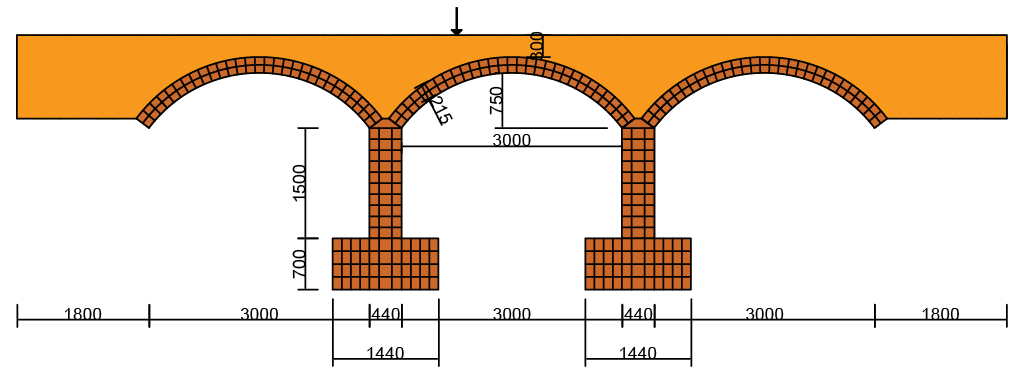
\includegraphics[width=0.95\linewidth]{./Figures/bridge_geometry.png}
\caption{Geometry of the three-span masonry arch bridge adopted for the scour application study.}
\label{fig:dmem-scour-geometry}
\end{figure}

The original laboratory campaign did not include a realistic foundation system. The piers were supported directly by the laboratory reaction structure, which can be interpreted as a rigid vertical support condition. For the present study, foundation plinths are introduced below the piers to represent a more realistic bridge configuration and to provide a mechanical location where support degradation can be imposed. The foundation dimensions and bridge geometry are shown in \Cref{fig:dmem-scour-geometry}.

The masonry, backfill, and interface material properties are adopted consistently with the validated model reported in \Cref{cha:dmem-validation}. This choice is important because the chapter aims to isolate the effect of foundation support degradation, not to recalibrate the masonry or backfill material response. The no-scour configuration is therefore treated as the baseline model against which all scour scenarios are compared.

\section{Soil--Foundation Interaction}
\label{sec:dmem-scour-foundation}

In the validation model, the bridge response was obtained using a rigid or quasi-rigid support condition. To investigate scour, this assumption is relaxed by introducing a Winkler-type vertical soil--foundation interface beneath the foundation plinths. The interface is represented by vertical springs distributed along the base of the foundation. These springs transmit compression between the foundation and the supporting soil and can be selectively removed to idealise erosion of the support.

The modulus of subgrade reaction is set to

\begin{equation}
k_s = 0.43~\mathrm{N/mm^3}.
\label{eq:dmem-scour-ks}
\end{equation}

This relatively high value is selected to approximate the quasi-rigid vertical restraint of the original benchmark while still allowing local support removal to be represented explicitly. A compressive stress limit is also assigned to the supporting soil,

\begin{equation}
q_c = 300~\mathrm{kN/m^2},
\label{eq:dmem-scour-qc}
\end{equation}

to prevent unrealistically high local contact stresses beneath reduced support widths. This value represents a simplified bearing resistance for a competent granular support and should be interpreted as a modelling parameter rather than a site-specific geotechnical characterisation.

Two levels of modelling are considered. The first is a two-dimensional longitudinal configuration in which the three-dimensional bridge is reduced to a representative vertical slice. This model focuses on in-plane response and provides the residual-capacity curves used in the first part of the chapter. The second is a preliminary three-dimensional configuration used to explore transverse support loss and out-of-plane collapse mechanisms. The two models are treated separately because their scour descriptors and response quantities are not yet at the same level of maturity.

\section{Scour Modelling Strategy}
\label{sec:dmem-scour-strategy}

Scour is represented by progressive removal of the vertical soil--foundation interaction at the pier base. In the \gls{DMEM} model, this is implemented by deactivating the Winkler interface springs located beneath the eroded portion of the foundation. The approach is intentionally idealised, but it provides a clear and reproducible way to connect support loss to structural response.

\begin{figure}[htbp]
\centering
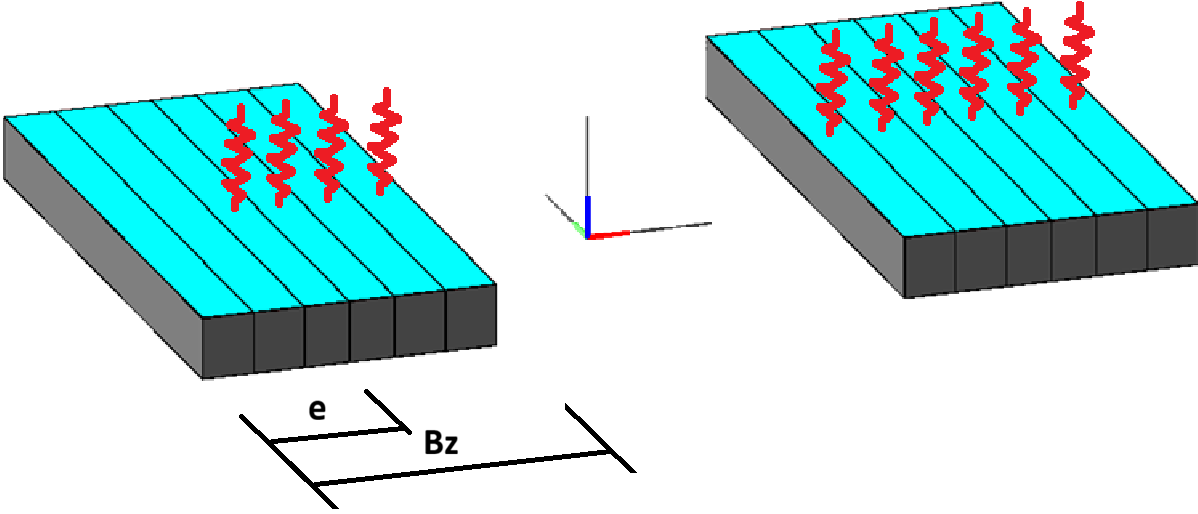
\includegraphics[width=0.75\linewidth]{./Figures/Interface_removed_e_Bz.png}
\caption{Idealised removal of soil--foundation interface elements used to represent local scour at one side of a pier foundation.}
\label{fig:dmem-scour-interface-removal}
\end{figure}

The severity of support loss is quantified through dimensionless scour ratios. For longitudinal, in-plane scour, the ratio is defined as

\begin{equation}
\eta_{s,x} = \frac{e_x}{B_x},
\label{eq:dmem-scour-ratio-x}
\end{equation}

where $e_x$ is the erosion length measured along the bridge longitudinal direction and $B_x$ is the corresponding foundation plinth dimension. For transverse, out-of-plane scour, the equivalent ratio is

\begin{equation}
\eta_{s,y} = \frac{e_y}{B_y},
\label{eq:dmem-scour-ratio-y}
\end{equation}

where $e_y$ is the erosion length measured across the bridge width and $B_y$ is the foundation width in that direction. The scalar notation \gls{eta_s} is retained when the direction is clear from the context. For a given value of the relevant ratio, the springs located within the eroded part of the foundation are removed, while the springs inside the remaining supported region continue to transmit compression. The parameters $\eta_{s,x}$ and $\eta_{s,y}$ are therefore structural support-loss indices rather than hydraulic scour-depth variables. A future diagonal scour case can be represented by combining non-zero values of both ratios, but that coupled case is not analysed in the present chapter.

\section{Analysis Procedure}
\label{sec:dmem-scour-analysis-procedure}

The nonlinear analyses follow a staged procedure. First, the bridge is brought to equilibrium under self-weight. This establishes the initial stress state in the masonry, backfill, foundations, and soil--foundation interface.

Second, scour is applied by removing interface springs according to the selected scenario and value of $\eta_{s,x}$ or $\eta_{s,y}$. The analysis is then iterated until a new equilibrium configuration is reached. This phase allows foundation settlement, pier rotation, and internal force redistribution to develop before traffic loading is applied.

Third, a vertical load is applied incrementally at one quarter of the central span. This load position follows the benchmark validation setup and provides a consistent basis for comparing residual capacity between scour scenarios. The maximum load factor sustained by the bridge is recorded as the residual load-carrying capacity for that scour configuration.

This staged procedure is important because it separates the structural consequences of support degradation from the subsequent live-load capacity. It also reflects the physical sequence expected in practice: scour modifies the support condition first, and the bridge then carries traffic loads in a degraded configuration.

\input{\currfiledir p_delta_scour_wall_validation}

\section{Baseline No-Scour Response}
\label{sec:dmem-scour-baseline}

Before assessing scour scenarios, the model with the soil--foundation interface is compared against the benchmark response of the original validated model and the experimental results. This comparison verifies that the introduction of the Winkler interface does not substantially alter the bridge response when no scour is present.

\begin{figure}[htbp]
\centering
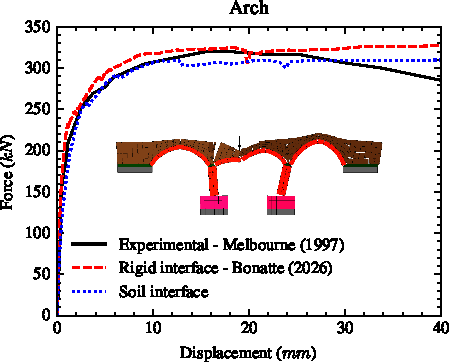
\includegraphics[width=0.78\linewidth]{./Figures/arch_benchmark.pdf}
\caption{Arch load-displacement response for the no-scour configuration, compared with experimental and rigid-interface benchmark results.}
\label{fig:dmem-scour-arch-benchmark}
\end{figure}

\begin{figure}[htbp]
\centering
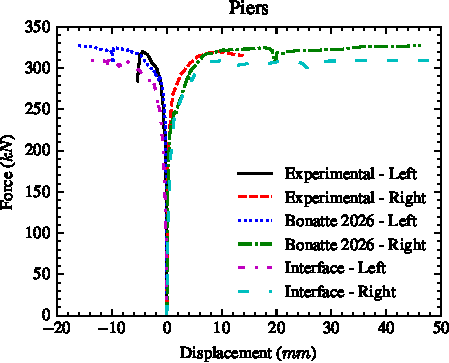
\includegraphics[width=0.78\linewidth]{./Figures/piers_benchmark.pdf}
\caption{Pier displacement response for the no-scour configuration, compared with experimental and rigid-interface benchmark results.}
\label{fig:dmem-scour-pier-benchmark}
\end{figure}

\Cref{fig:dmem-scour-arch-benchmark,fig:dmem-scour-pier-benchmark} show that the soil-interface model remains close to the experimental and benchmark numerical responses. The no-scour capacity is not significantly affected by the introduction of the foundation interface, while the model gains the ability to represent foundation-level deformability and support degradation. This confirms that the soil-interface model can be used as the reference configuration for the scour analyses.

\subsection{Parametric study - Influence of geometrical parameters}

% \cite{Tubaldi2020_MesoscaleMAB} has done the following:

% - location of the vertical load normalized with respect to the span length (l/s)
%   * Fig. 10c illustrates the influence of the location of the vertical load on the bridge capacity and collapse mechanism. The highest capacity corresponds to a load located at 3/4 of any of the two side spans, whereas the lowest is found for a load located at the middle of the central span.

% - influence of the number of spans on the collapse load
%   * Fig. 10d shows the influence of the number of spans on the collapse load. The bridge capacity decreases significantly by increasing the number of spans from 1 to 3, while for a number of spans higher than 3 it remains practically constant. This is consistent with the fact that at most two spans are involved in the collapse mechanism, as observed both in Fig. 14 and in Fig. 2.

% The trend of variation with the loading position is such that the lowest resistance is found when the load is applied at the middle of the external or central span, whereas it is highest when the load is closer to the pier, as expected. The collapse load also reduces significantly by passing from the single span bridge to the three-span bridge.

% I also have to review {Oliveira2010} for the geometric issues.
% For medium spans, the critical location of the central axle is roughly at the 1/5 span of the bridge for semi-shallow arches (bridge C) and at about the 1/3 span for deep arches (bridge D).

% One thing that they did not do was to consider the load location when there is scour on the pier.

%%TODO
% I can add for both (in-plane and out-of-plane) a influence line diagram.
% I mean, I can run the analysis for different scour scenarios.
% Calculate the most unfavorable position.
% I can use this for future justify the load location.
% It is expected to be 1/4 or 1/2 of the span.
% I can also see if the location change depending on the scour scenario.

% MAURI-003 TODO -- load-position sensitivity plan.
% Add a later subsection, before the in-plane/out-of-plane result blocks, to
% justify the adopted live-load position with a small influence-line or moving-
% load sensitivity study.
% Proposed analysis:
% - run the validated no-scour model and selected scour scenarios with the live
%   load placed at several positions along the span;
% - repeat the sweep for both in-plane and out-of-plane support-loss cases;
% - extract residual capacity, governing displacement, and collapse mechanism;
% - identify whether the most unfavourable position is near quarter-span,
%   mid-span, or changes with the scour location/intensity;
% - use the result to justify the fixed load location used in this chapter and
%   to define load-position variables for later surrogate/reliability work.

%%TODO
% I have to separete my analysis in two categories.
% One that only considers the dead load. This is probably the most commom cases of bridge collapse. They collapse during a flood without additional load.
% The second analysis is the collapse with scour by a live load. This is very critial because it involves actual people on the bridge.

\input{\currfiledir in_plane}
\input{\currfiledir out_of_plane}

\section{Limitations and Future Work}
\label{sec:dmem-scour-limitations}

The present application is intentionally simplified and should be interpreted as a mechanistic study. The main limitations are:

\begin{enumerate}
    \item the soil is represented by a Winkler-type vertical interface rather than by a continuum or nonlinear geotechnical model;
    \item the scour process is represented by support removal, not by a coupled hydraulic--geotechnical erosion simulation;
    \item the live load is applied at a fixed position, whereas moving train or traffic loads may activate different critical mechanisms;
    \item the out-of-plane results are preliminary and currently interpreted qualitatively;
    \item the material and geometric uncertainties are not yet propagated through the model.
\end{enumerate}

Future work should therefore extend the analysis to multiple load positions, moving load models, material and geometric sensitivity analysis, coupled longitudinal--transverse scour patterns, and probabilistic descriptions of scour development. These developments will allow the residual-capacity curves obtained here to be incorporated into the broader PhD framework for vulnerability, risk, resilience, and decision-making.

\section{Chapter Conclusions}
\label{sec:dmem-scour-conclusions}

This chapter applied the validated \gls{DMEM} strategy to investigate scour-induced capacity degradation in a representative three-span masonry arch bridge. Scour was idealised as staged removal of soil--foundation support and quantified through dimensionless support-loss ratios, with $\eta_{s,x}$ describing longitudinal removal and $\eta_{s,y}$ describing transverse removal.

The in-plane analyses show that the effect of scour is highly scenario-dependent. Overbank-side scour at the left-bank pier is the controlling case for the analysed bridge and load position, leading to progressive capacity reduction. Channel-side scour is non-critical in the examined configurations because that side of the foundation tends to unload during the governing pier-rotation mechanism. Combined scour at both piers does not necessarily reduce capacity beyond the critical single-pier scenario, because collapse localises before the second pier is significantly mobilised.

The preliminary out-of-plane analyses indicate that transverse support loss can activate a different deformation pattern, with asymmetric displacement and interface-stress redistribution across the foundation width. These results are not yet used to define numerical fragility parameters, but they establish the modelling basis for later three-dimensional and diagonal scour scenarios.

The study confirms that the validated \gls{DMEM} model can be used not only for vertical-load assessment but also for investigating flood-induced boundary-condition degradation. This makes the chapter a bridge between the numerical validation work and the later PhD tasks on flood vulnerability, fragility, and resilience-based decision support.



% I must follow \cite{Scozzese2023} adivice:
% "
% Considering the substantial similarity in shape and size of the bridges
% falling into the class of structures analysed in this paper, it is expected that the response and the behaviour observed in the present case study under scour actions can be also representative of other similar contexts, at least from a qualitative point of view, while it may be possible, for instance, to observe other bridges failing for lower values of Bs/B. Hence, it may be advisable to extend the study considering bridges with other geometrical and mechanical properties, which reveals a necessary step for the aim, for instance, of developing scour fragility functions for this bridge typology. The provided recommendation about the param- eters to be monitored and the optimal sensors location, instead, are expected to be general.
% "
